\documentclass{article}

\usepackage[utf8]{inputenc}
\usepackage[T1]{fontenc}
\usepackage[french]{babel}
\usepackage{graphicx}
\usepackage{subfigure}
\usepackage{anysize}
\usepackage{wrapfig}
\usepackage{colortbl}
\usepackage{fancyhdr}
\usepackage{mathtools}
\usepackage{smartdiagram}
\usepackage{tikz}
\usetikzlibrary{arrows,shapes,positioning,shadows,trees}

\tikzset{
  basic/.style  = {draw, text width=2cm, drop shadow, font=\sffamily, rectangle},
  root/.style   = {basic, rounded corners=2pt, thin, align=center,
                   fill=yellow!30},
  level 2/.style = {basic, rounded corners=6pt, thin,align=center, fill=green!30,
                   text width=8em},
  level 3/.style = {basic, thin, align=left, fill=gray!60, text width=6.5em}
}

\pagestyle{empty}
    
\marginsize{2.5cm}{2.5cm}{2.5cm}{2.5cm}
\fancyhead[RO,LE]{Le grand Londres}
\fancyhead[RE,LO]{ASRALL 2017 - \LaTeX}
\fancyfoot[LO,LE]{-Rosendo Bonilla Juárez-}

\begin{document}

\newpage
\begin{titlepage}
\begin{figure}[ht]
\begin{center}
\vspace{1.5cm}
% Aquí se inserta un escudo o emblema:

\includegraphics[scale=1.2]{./images/logo.jpg}
\label{escudouam1}
\vspace{-1cm}
\end{center}
\end{figure}
\begin{center}


\vspace{2.3cm} {\LARGE ASRALL}

%------------------------------------------------------

\vspace{1.5cm} {\Huge LE GRAND LONDRES}

\begin{figure}[ht]
\begin{center}
\vspace{0.8cm}


\includegraphics[scale=0.6]{./images/london.jpg}
\label{logo}
\vspace{-1cm}
\end{center}
\end{figure}

\vspace{1.8cm} Nancy, 2017
\end{center}
\end{titlepage}

%-------------------------------------------------------

\newpage
\vspace*{\fill}
\begin{flushright}\Huge{\textbf{Le grand Londres}}\end{flushright}
\vspace*{\fill}

\newpage

\vspace*{\fill}
\begin{flushleft}

\huge{\textbf{À Londres au crépuscule}}
\ \\ \ \\
\small{\textit{Francis Etienne Sicard}}

\ \\ \ \\
Les rues en diamants et leur soyeux pavage,\\
Comme des serpentins lâchés des toits obscurs,\\
Glissent, de pas en pas, le long de mers de murs,\\
Tapissés du soleil de vitrine en voyage.
\ \\ \ \\
Un bus à impériale et son rouge ramage\\
Croise une limousine aux fourreaux de noirs purs,\\
L’un éteignant le jour et ses rêves d’azurs,\\
L’autre incendiant la nuit d’une ivresse volage.
\ \\ \ \\
La Tamise soudain se pare de colliers,\\
Et Big Ben se maquille à l’or de ses aiguilles,\\
Chuchotant des dîners, fards des joailliers.
\ \\ \ \\
La magicienne alors entre de scène en scène\\
Soulevant les rideaux dont les tons de charmilles\\
Font frissonner la ville aux plaisirs des mécènes.\\
\end{flushleft}
\vspace*{5mm}


\newpage    
\tableofcontents
\newpage
\setcounter{page}{1}
\pagestyle{fancy}
\section{Introduction}

\begin{wrapfigure}{r}{0.4\linewidth}
\centering
\subfigure{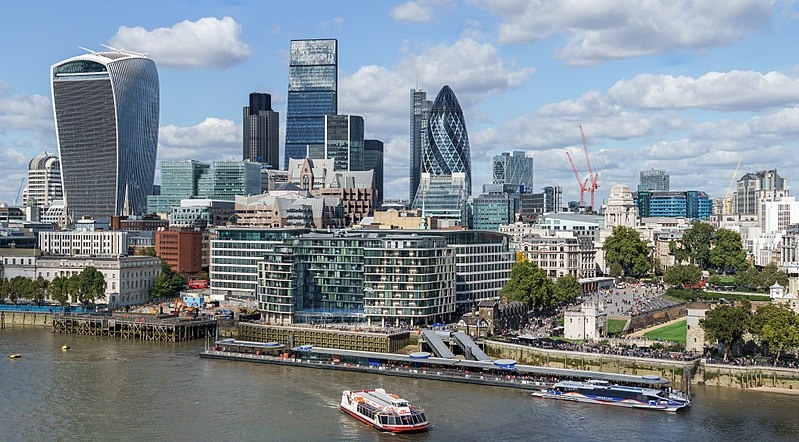
\includegraphics[width=55mm]{./images/un.jpg}}
\subfigure{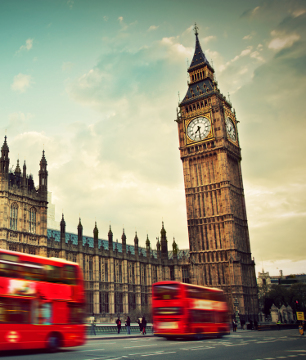
\includegraphics[width=27mm,height=29mm]{./images/deux.jpg}}
\subfigure{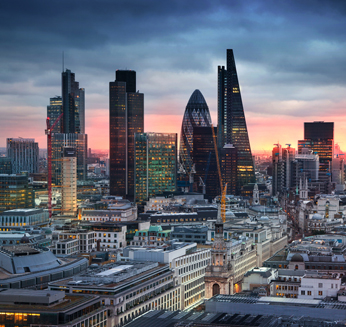
\includegraphics[width=27mm,height=29mm]{./images/trois.jpg}}
\subfigure{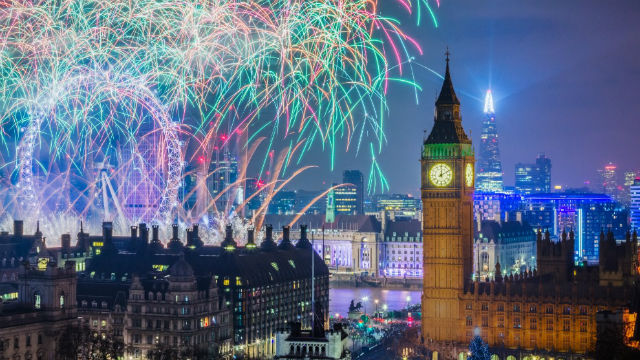
\includegraphics[width=55mm]{./images/cinq.jpg}}
\begin{tabular}{>{\columncolor[gray]{0.8}}l|>{\columncolor[rgb]{0.9,0.8,0.5}}r}
    \hline    
    \multicolumn{2}{>{\columncolor[rgb]{0.8,0.9,0.1}}c}{Administration}\\
    \hline
    Pays & Royaume-Uni\\
    \hline
    Nation & Angloterre\\
    \hline
    Région & Londres\\
    \hline
    Comté & Cité et Grand Londres\\
    \hline    
    District & Cité et 32 districts\\
    \hline    
    \multicolumn{2}{>{\columncolor[rgb]{0.8,0.9,0.1}}c}{Démographie}\\
    \hline
    Gentilé & Londonien\\
    \hline
    Pop. & 8 673 713 hab.\\
    \hline
    Densité & 5 518 hab./km2\\
    \hline
\end{tabular}
\caption {Info. générale.} \label{fig:intro}
\end{wrapfigure}

Londres, située dans le sud-est de la Grande-Bretagne, est la capitale et la plus grande ville de l'Angleterre et du Royaume-Uni. Longtemps capitale de l'Empire britannique, elle est désormais le siège du Commonwealth of Nations (\textbf{voir Figure ~\ref{fig:intro}}).

Fondée il y a presque 2 000 ans par les Romains sous le nom de Londinium, Londres était au XIXe siècle la ville la plus peuplée du monde. Bien que largement dépassée dans ce domaine par de nombreuses mégapoles, elle reste une métropole de tout premier plan2, en raison de son rayonnement et de sa puissance économique, dû notamment à sa place de premier centre financier mondial3. Londres se place dans le rang des grands centres financiers et culturels du monde avec New York et Hong Kong, cette trilogie est appelée par les médias anglophones "Nylonkong".

La région de Londres, composée de l'Inner London et de l'Outer London, comptait environ 8 673 000 habitants en 2015 et réalise un cinquième du produit intérieur brut du Royaume-Uni5. En 2015, l'aire urbaine de Londres comptait 9 787 426 habitants et son aire métropolitaine 12 317 800 habitants. En Europe, seules les agglomérations de Moscou, Istanbul et Paris6 ont un poids démographique comparable. Ses habitants s'appellent les Londoniens (en anglais : Londoners).

Londres, la seule ville du monde à ce jour à avoir organisé trois fois les Jeux olympiques (1908, 1948, 2012), est dynamique et très diverse sur le plan culturel. Elle joue un rôle important dans l'art et dans la mode. Elle reçoit 28 millions de touristes par an et compte quatre sites inscrits au patrimoine mondial ainsi que de nombreux monuments emblématiques : le Palais de Westminster, le Tower Bridge, la Tour de Londres, l'Abbaye de Westminster, le Palais de Buckingham, ainsi que des institutions renommées comme le British Museum ou la National Gallery.

C'est faux, répond Le Monde. Si aucun chiffre exact n'est publié, les Français n'étant pas obligés de s'enregistrer au sein de l'Union européenne, le consulat de France estime qu'"au moins 300.000 Français" sont installés au Royaume-Uni, dont les trois quarts vivent dans le grand Londres. Soit 225.000 personnes.

Un chiffre à peine inférieur à celui avancé par le maire de Londres. Mais Le Monde estime que ce nombre placerait Londres "au trentième rang des agglomérations françaises".
Il y a 8,6 millions habitants dans ce qu'on appelle le Grand Londres, soit quatre plus qu'à Paris. La ville est très vaste et  s'étend sur près de 1.600 km2, soit 15 fois plus que Paris, mais il faut savoir que Londres a absorbé sa banlieue dans les années 60. Cela dit, la capitale britannique est un véritable champignon démographique puisque 100.000 nouveaux habitants y arrivent chaque année, parmi lesquels énormément d'étrangers. Les Français seraient environ 200.000 à Londres. 

%latexmk -pvc londres

\newpage


\section{Géographie}
\subsection{Définition de Londres}

La dénomination courante Londres peut désigner plusieurs ensembles géographiques ou administratifs différents, pouvant parfois porter à confusion (\textbf{Figure~\ref{fig:geo1}}).

L'emploi le plus courant fait référence au Grand Londres (Greater London), une des neuf subdivisions régionales de l'Angleterre, formé du territoire sous l'autorité du Greater London Authority et du maire de Londres. Le Grand Londres est considéré comme une région NUTS-1 au sein de l'Union européenne. C'est cet ensemble d'environ 1 600 km2 pour 7,5 millions d'habitants qui est couramment désigné lorsque l'on parle de la capitale britannique. Le Grand Londres est divisé en deux zones, Inner London et Outer London. 
\begin{wrapfigure}{l}{0.4\linewidth}
\centering
\subfigure{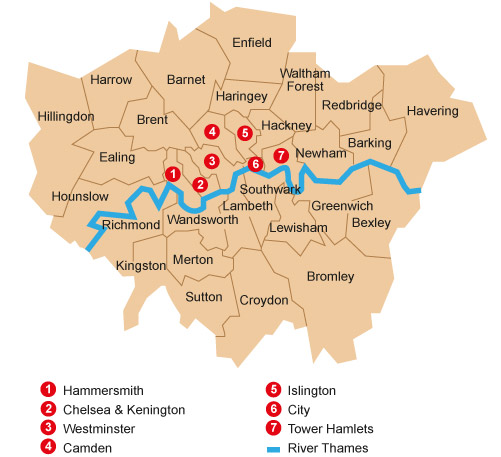
\includegraphics[width=55mm]{./images/geo.jpg}}
\caption{Carte de la ville}
\label{fig:geo1}
\end{wrapfigure}
Les deux zones sont considérées des régions NUTS-2. Cependant, le Grand Londres n'est pas officiellement une cité, dont le statut, strictement défini au Royaume-Uni, est attribué à une ville par le monarque britannique sur des critères précis. Avant sa création en 1965, le territoire du Grand Londres faisait partie des comtés du Kent, Middlesex, Surrey, Essex et du Hertfordshire.
La cité de Londres (City of London, abrégé en City, ou bien Square Mile en référence à sa superficie de 1 mile carré), située au cœur du Grand Londres, correspond à la définition historique de Londres. C'est là que la ville moderne est née et c'est aujourd'hui le plus ancien quartier de la capitale. C'est également une circonscription à part entière avec un statut spécial. La cité de Londres et le reste du Grand Londres forment deux régions dites de « lieutenance » (Lieutenancy areas) différentes.
La vaste agglomération londonienne peut être décrite par la région urbaine de Londres, qui correspond à la zone occupée par les banlieues, et qui occupe un territoire à peu près similaire à la région du Grand Londres mais avec une population légèrement supérieure. Au-delà de la région urbaine se trouve l'aire urbaine de Londres (London commuter belt ou London Metropolitain Area) qui regroupe les territoires habités par des personnes se déplaçant quotidiennement (commuters) pour aller travailler à Londres. La région urbaine de Londres s'est considérablement agrandie durant l'époque victorienne puis de nouveau pendant l'entre-deux-guerres. Son expansion s'est arrêtée dans les années 1940 à cause de la Seconde Guerre mondiale et de la politique dite de la ceinture verte et sa superficie n'a pas beaucoup évolué depuis. Les limites du district de la Metropolitan Police et de la zone desservie par les transports londoniens ont évolué au fil du temps mais correspondent aujourd'hui approximativement à celle du Grand Londres.
\subsection{Relief et hydrographie}
Le Grand Londres se situe à 50 km à l'ouest de l'estuaire de la Tamise et s'étend sur une superficie de 1 579 km2 (37e rang mondial9). L'altitude y varie du niveau de la mer jusqu'à 245 m, Biggin Hill, au sud de l'agglomération (\textbf{voir Figure~\ref{fig:geo2} dans la page~\pageref{fig:geo2}}).\\

Le fleuve, qui traverse la ville d'ouest en est, a eu une influence majeure sur le développement de la ville. Londres a été fondée à l'origine sur la rive nord de la Tamise et n'a disposé, pendant plusieurs siècles, que d'un seul pont, le pont de Londres (London Bridge). Le foyer principal de la ville s'est en conséquence cantonné sur cette rive de la Tamise, jusqu'à la construction, au XVIIIe siècle, d'une série d'autres ponts. La ville s'est alors étendue dans toutes les directions, cette expansion n'étant gênée par aucun obstacle naturel, dans une campagne presque dépourvue de reliefs, à l'exception de quelques collines (Parliament Hill, Primrose Hill).
\newpage

\begin{wrapfigure}{r}{0.4\linewidth}
\centering
\subfigure{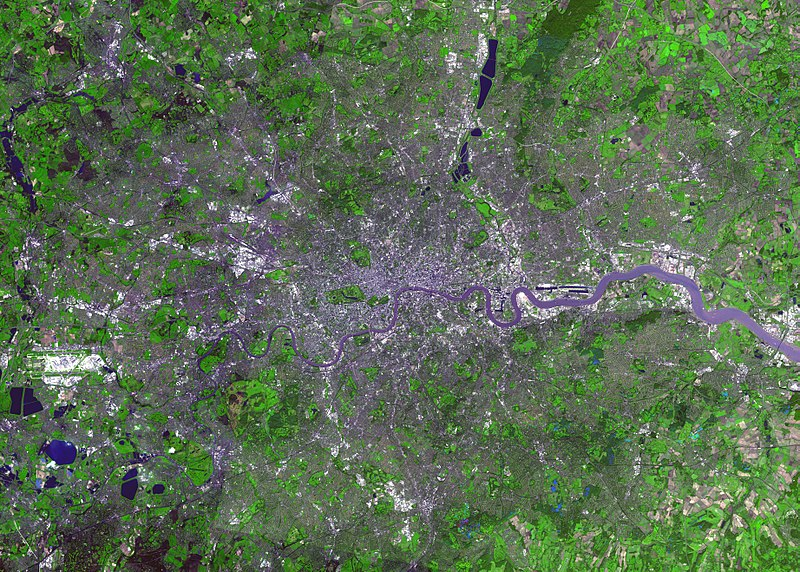
\includegraphics[width=55mm]{./images/relief.jpg}}
\caption{Vue satellite}
\label{fig:geo2}
\end{wrapfigure}
La Tamise était autrefois plus large et moins profonde qu'aujourd'hui. Les rives du fleuve ont été massivement aménagées, la plupart des affluents ont été détournés et sont à présent souterrains, parfois transformés en égouts (ainsi, la rivière Fleet dont le nom subsiste dans Fleet Street, l'ancienne rue des journaux). La Tamise est sujette à la marée et Londres est largement inondable. Les menaces d'inondation augmentent d'ailleurs avec le temps compte tenu de l'élévation régulière du niveau de l'eau à marée haute et de la lente inclinaison de la Grande-Bretagne (relèvement au nord, abaissement au sud) causée par un phénomène de relèvement isostatique. Un barrage, la Barrière de la Tamise, a été construit à travers la Tamise à Woolwich dans les années 1970, pour pallier cette menace. En 2005 cependant, il a été suggéré la construction d'un barrage d'une quinzaine de kilomètres de long plus en aval afin de parer les risques futurs d'inondation.

\subsection{Quartiers}
On décrit souvent Londres par quartiers (Bloomsbury, Mayfair, Whitechapel par exemple). Ces noms n'ont pas d'utilisation officielle mais désignent souvent des paroisses (parishes) ou des circonscriptions (city wards) et sont restés en usage par tradition, chacun faisant référence à un quartier distinct avec ses propres caractéristiques mais sans délimitation officielle.

Il existe cependant une zone centrale de Londres qui possède une définition et un statut stricts, la Cité de Londres (City of London). Souvent appelée simplement la City, c'est l'un des plus grands quartiers financiers (central business district) mondiaux. La City possède son propre corps gouvernant et ses propres frontières, lui donnant ainsi une complète autonomie politique et administrative. Le nouveau quartier financier et commercial des docklands se situe à l'est de la City et est dominé par Canary Wharf. L'autre quartier d'affaires se trouve dans la Cité de Westminster qui abrite également le gouvernement britannique et l'Abbaye de Westminster.

\subsection{Climat}

Le climat de Londres symbolise parfaitement le climat de type océanique. Les précipitations sont régulières toute l'année souvent sous forme de bruine, contrairement à l'ouest du Royaume-Uni où elles sont d'intensité plus forte. La moyenne annuelle des précipitations s'établit à 622,5 mm, février étant le mois le plus sec de l'année. Ce niveau est inférieur à Rome ou Sydney. Londres est en fait une des capitales européennes les plus sèches, disposant de ressources d'eau par personne inférieures à celles d'Israël par exemple, l'impression de temps maussade vient surtout du fait que l'ensoleillement annuel est faible. Des villes aussi pluvieuses mais avec un ensoleillement élevé ne provoquent pas cette impression de temps maussade qu'on trouve à Londres.

Les étés sont tempérés, les jours de fortes chaleurs sont rares et les hivers sont froids mais rarement glaciaux. Le mois le plus chaud est juillet avec une température moyenne à Kew Gardens de 18.0 C n'excédant que rarement les 33, quoique des niveaux plus élevés soient devenus plus fréquents récemment, les températures estivales en journée varient généralement entre 20 et 25 C. La plus haute température fut de 38,1 C, mesurée dans les jardins botaniques royaux de Kew, le 10 août 2003, pendant la canicule de 2003. Le mois le plus froid est janvier avec des températures moyennes de 2,4 C à 7,9 C. La température la plus froide fut de -16,1 C, le 1er janvier 1962 à Northolt.

Les chutes de neige abondantes sont presque inconnues. Au cours des hivers les plus récents, la neige a rarement excédé un pouce d'épaisseur (soit moins de 3 cm). Ceci est notamment dû au fait que la vaste agglomération londonienne crée un microclimat, avec une chaleur enfermée par les immeubles de la ville. La nuit, la température y est parfois de 5 à 9 C supérieure aux zones environnantes. Le célèbre smog londonien, mélange de brouillard et de fumée, est devenu rarissime dans les rues de la capitale anglaise. En 1954, il avait provoqué la mort de 4 000 personnes (\textbf{voir Table~\ref{climat} dans la page~\pageref{climat}}).
%>{\columncolor[gray]{0.8}}   >{\columncolor[rgb]{0.9,0.8,0.5}}

\begin{table}
\begin{center}
\resizebox{16cm}{!}{
\begin{tabular}{|>{\columncolor[gray]{0.8}}c|c|c|c|c|c|c|c|c|c|c|c|c|}
    \hline
    \rowcolor[gray]{0.8}Mois&jan.&fév.&mars&avril&mai&juin&jui.&août&sep.&oct.&nov.&déc. \\
    \hline    
    Température minimale moyenne (C) &\cellcolor[rgb]{0,1,1}1,8 &\cellcolor[rgb]{0,1,1}1,7 & 3,4 & 4,7 & 7,9 & 10,8 & 13 &17&10,3&7,4&5&12,3\\
    \hline
    Température moyenne (C) & 2,8 & 4,7 & 1,4 & 2,7 & 3,4 & 10,2 & 14 &1,7&1,5&4,4&5&15,2\\
    \hline
    Température maximale moyenne (C) & 3,8 & 1,2 & 4,3 & 2,9 &\cellcolor{red}17,9 &\cellcolor{red}19,8&\cellcolor{red}26,0&\cellcolor{red}20,0&12,6&9,5&4&11,2\\
    \hline    
    Ensoleillement (h) & 3,2 & 2,6 & 8,3 & 2,4 & 5,7 & 12,1 & 12 &17,4&10,2&7,2&2,5&11,3\\
    \hline
    Précipitations (mm) & 5,2 & 1,4 & 4,2 & 7,9 & 1,2 & 12,4 & 1,3 &1,4&11,5&9,4&4,5&11,5\\
    \hline    
\end{tabular}
}
\end{center}
\caption{Relevé météorologique de Londres Kew Gardens (période : 1981-2010)}
\label{climat}
\end{table}
\ \\ \ \\

\newpage
\section{Histoire}
\subsection{Londres à l'époque romaine}

Les régions aux alentours de Londres (aujourd'hui situées à l'intérieur des frontières du Grand Londres) tissent une première ville24. Ce premier campement est appelé Londinium. Le pont de Londres se trouvait au centre du tout nouveau réseau de routes créé par les Romains et était un lieu de passage privilégié pour traverser la Tamise, ce qui a attiré de nombreux commerçants et ainsi contribué à la croissance de la ville. Londres est vite devenue un important centre d'échanges et de commerce, la Tamise permettant d'acheminer facilement des marchandises jusqu'au cœur de la ville).

\begin{wrapfigure}{r}{0.4\linewidth}
\centering
\subfigure{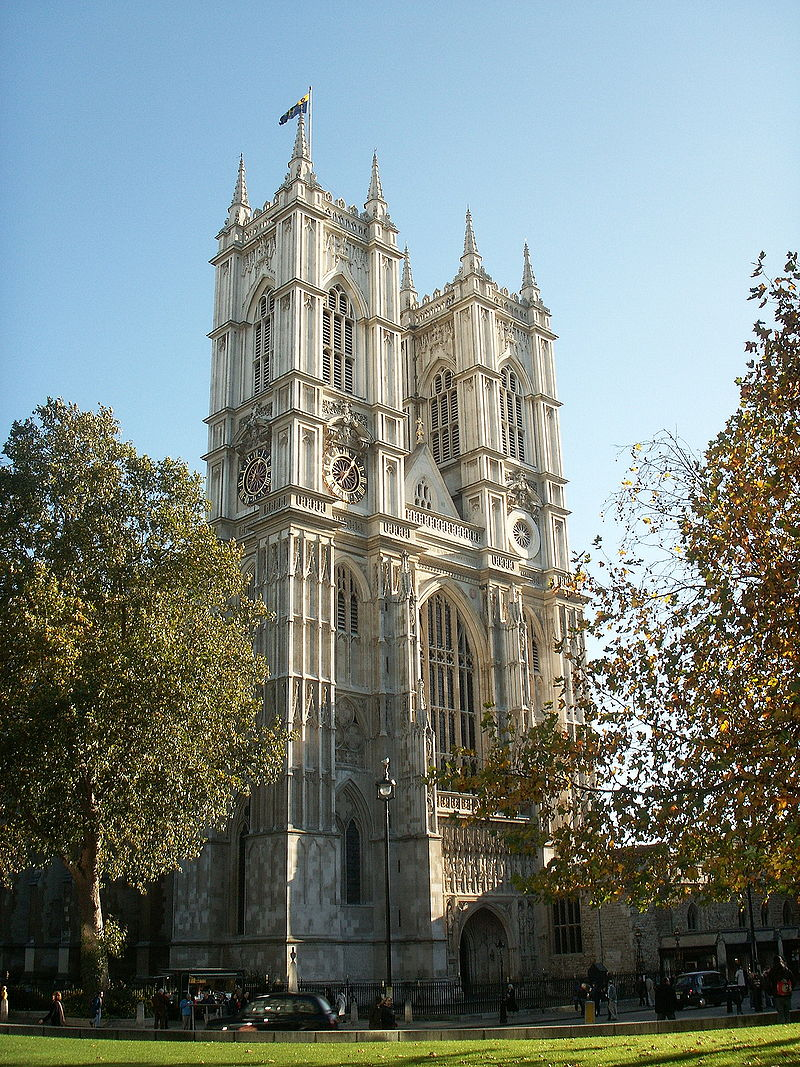
\includegraphics[width=50mm]{./images/hist1.jpg}}
\caption{Abbaye de Westminster}
\label{fig:hist1}
\end{wrapfigure}

\subsection{Londres médiévale}
La position privilégiée de la ville sur la Tamise en fait un lieu stratégique et vers l'an 600, les Anglo-Saxons fondent une nouvelle ville, Lundenwic, à environ 1 km en amont de la ville romaine, à l'endroit où se trouve aujourd'hui Covent Garden. Un port de pêche et de commerce est probablement localisé à l'embouchure de la rivière Fleet. Lundenwic prospère jusqu'en 851, lorsque la ville est envahie et complètement rasée par les Vikings. Après cette occupation viking, Alfred le Grand rétablit la paix et fait déplacer la ville dans les murailles de la vieille cité romaine (alors appelée Lundenburgh) en 886. La ville originale est devenue Ealdwic (« vieille ville »), dont le nom a survécu jusqu'à aujourd'hui pour donner Aldwych.
Après la bataille d'Hastings, le duc de Normandie Guillaume le Conquérant est couronné roi d'Angleterre dans la toute nouvelle Abbaye de Westminster, le jour de Noël 1066. Il accorde certains privilèges aux habitants de Londres tout en construisant un château au sud-est de la ville pour maintenir le contrôle sur la population. Ce château, agrandi par les rois suivants, sert de résidence royale puis de prison et est aujourd'hui connu sous le nom de Tour de Londres.
En 1097, Guillaume le Roux commence la construction du Hall de Westminster, près de l'abbaye du même nom. Ce hall est à l'origine du palais de Westminster, la résidence royale tout au long du Moyen Âge. Westminster devient le siège de la cour royale et du gouvernement, tandis que la Cité de Londres voisine forme un centre d'échanges et de commerce prospère sous l'autorité de sa propre administration, la Corporation of London. Les villes aux alentours se développent et forment la base du cœur de Londres moderne, remplaçant Winchester en tant que capitale du royaume d'Angleterre au XIIe siècle.
Le 2 juin 1216, Le prince Louis (futur Louis VIII) s'empare de la ville jusqu'en 1217.


\subsection{L'époque contemporaine}
De 1825 à 1925, Londres est la ville la plus peuplée au monde. Cette croissance est accélérée par la construction des premières lignes de chemin de fer à Londres, rapprochant considérablement les villes avoisinantes. Porté par un essor boursier exceptionnellement rapide, ce réseau ferroviaire s'étend rapidement et permet à ces villes de croître tout en permettant à Londres de s'étendre et d'englober les villages aux alentours, à l'image de Kensington. L'apparition des premiers embouteillages en centre-ville mène à la création, en 1863, du premier système de transport souterrain au monde, le métro de Londres, accélérant encore le développement de l'urbanisation29. Grâce à cette croissance rapide, Londres devient l'une des premières villes à dépasser le million d'habitants et la première à dépasser les cinq millions.

Le gouvernement local de Londres éprouve des difficultés à gérer l'expansion rapide de la ville, surtout au niveau des infrastructures. Entre 1855 et 1889, le Metropolitan Board of Works supervise la croissance des infrastructures. Il est remplacé par le comté de Londres, géré par le London County Council, la première assemblée élue au niveau de la ville, jusqu'en 1965.

\newpage

\section{Démographie}

Londres a toujours été un important foyer de population. À la fois, ville, aire urbaine et région urbaine la plus peuplée du Royaume-Uni, elle a également été la plus peuplée d'Europe et du monde avant de connaître un léger déclin.


\subsection{Population}
Le Grand Londres, composé de Inner London et Outer London, compte 8 615 000 habitants en 2014. L'aire urbaine de Londres compte près de 10 millions d'habitants tandis que l'aire métropolitaine, sa zone d'influence directe, compte 15 millions d'habitants. D'après Eurostat, Londres est la première ville la plus peuplée et la deuxième aire urbaine la plus importante de l'Union européenne après Paris42. La ville se classe également au quinzième rang des villes les plus peuplées du monde et au quinzième rang des aires urbaines les plus peuplées.

La région du Grand Londres occupe une superficie de 1 572 km2 et la densité de population est de 5 285 habitants par km2, soit une densité plus de 10 fois supérieure à celle de l'Écosse, de l'Irlande du Nord, du pays de Galles ou de n'importe quelle autre région anglaise. Cette densité cache cependant des disparités au sein de 32 districts. En 2005, le borough royal de Kensington et Chelsea (Inner London) comptait 16 178 hab./km2 contre 2 011 pour Bromley (Outer London)43.

\begin{table}
\begin{center}
\resizebox{10cm}{!}{
\begin{tabular}{|l|r|}
    \hline
    Pays de naissance & Population (2011) \\
    \hline
    
\includegraphics[width=4mm]{./images/ru.png} Royame Uni & 5 175 677\\
    \hline    
    
\includegraphics[width=4mm]{./images/ind.png} Inde & 262 247\\
    \hline 
    
\includegraphics[width=4mm]{./images/pol.png} Pologne & 158 300\\
    \hline 
    
\includegraphics[width=4mm]{./images/irla.png} Irlande & 129 807\\
    \hline 
    
\includegraphics[width=4mm]{./images/nig.png} Nigeria & 114 718\\
    \hline 
    
\includegraphics[width=4mm]{./images/pak.png} Pakistan & 112 457\\
    \hline     
\end{tabular}
}
\end{center}
\caption{Relevé météorologique de Londres Kew Gardens (période : 1981-2010)}
\label{pop}
\end{table}


La structure de la population de Londres est légèrement différente de celle de l'Angleterre ou du Royaume-Uni. L'attractivité de Londres a entraîné une immigration vers la capitale de personnes en âge de travailler depuis le reste du pays ou l'étranger. La proportion de personnes entre 20 et 44 ans représente 42,8\% contre 35,1 à l'échelle nationale. En contrepartie, la proportion de personnes âgées de 60 ans et plus (14,4 \%) est inférieure à la moyenne nationale (18,4 \%) (\textbf{voir Table~\ref{pop}}).

Les chiffres de l'Office for National Statistics montrent que le nombre de Londoniens nés à l'étranger atteignait 2 288 000 en 2006 contre 1 630 000 en 1997.

Le tableau ci-contre donne le pays de naissance des résidents de Londres en 2011, date du dernier recensement britannique.

\newpage
\section{Économie}
En 2014, Londres est la cinquième ville du monde en termes de PUB, et la première d'Europe devant Paris intramuros. Le Grand Londres réalise environ un quart du PIB du Royaume-Uni, et l'aire métropolitaine de Londres environ un tiers. La productivité est nettement supérieure à la moyenne nationale. Très fortement tertiarisée, Londres connaît une importante spécialisation dans la finance. La capitale britannique est la première place financière du monde et l'un des principaux centres d'affaires internationaux. 

\subsection{Attrativité}
L'économie de Londres s'est orientée vers les services beaucoup plus tôt que d'autres villes européennes, surtout après la Seconde Guerre mondiale. Le succès de Londres dans le secteur tertiaire s'explique surtout par plusieurs des facteurs :
\begin{itemize}
    \item l'anglais est une langue de communication internationale ;
    \item sa position de capitale de l'Empire britannique ;
    \item ses relations particulières avec les États-Unis et plusieurs pays d'Asie,
    \item sa position géographique qui permet à ses horaires de bureau de correspondre à ceux d'autres pays qui comptent pour 99 % du PNB mondial ;
    \item le droit anglais est le droit des contrats le plus utilisé en commerce international ;
    \item les infrastructures multiculturelles (écoles, lieux de culte, organisations culturelles et sociales) ;
    \item un niveau d'impôt relativement peu élevé surtout pour les étrangers (les résidents non domiciliés au Royaume-Uni ne payent pas de taxe sur les profits réalisés à l'étranger) - cependant, la taxe du comté (équivalent de la taxe d'habitation française) payée chaque mois est très élevée (environ 100-150 livres/mois/logement) ;
    \item de bonnes infrastructures de transport, surtout dans le trafic aéroportuaire ;
    \item une économie dérégulée avec peu d'intervention du gouvernement.
\end{itemize}

\subsection{Tourisme}

\textbf{Londres est une des principales destinations touristiques au monde. Ce secteur génère entre 280 00080 et 350 00081 emplois selon les sources. En 2008, les revenus du tourisme représentaient 10,5 milliards £82. En 2014, Londres a reçu 17,4 millions de touristes étrangers, pour un total d'environ 28 millions.}

\textit{Londres bénéficie de son statut de capitale anglophone en Europe et attire ainsi chaque année de très nombreux étudiants du continent venus apprendre la langue anglaise. Une importante économie du tourisme estudiantin s'est développée autour de cette manne, certains n'hésitant pas à en profiter par des pratiques à la limite de la légalité.}

Les principaux sites touristiques londoniens sont concentrés dans le \textsc{West End}, qui comprend les grands magasins d’Oxford Street, les théâtres, et les quartiers tels que \textsc{Soho, Covent Garden, Mayfair, Piccadilly Circus} et la place de Leicester Square. Les monuments les plus célèbres de Londres sont \textsc{le British Museum, la Tate Gallery, le Tate Modern, Madame Tussauds, les palais de Westminster et de Buckingham, l’Imperial War Museum, le Science Museum, la National Gallery, la National Portrait Gallery, la Tower Bridge, Big Ben, la Tour de Londres, London Eye, Cathédrale St Paul et Arsenal Football Club Museum}.

\newpage

\section{Mexique}
\subsection{Un peu de l'histoire de Mexique}
\ \\ 
\begin{center}
\smartdiagram[descriptive diagram]{
  {1810,{Independance de Mexique de l'Espagne}},
  {1862, {Bataille de Puebla contre la France}},
  {1910, Révolution de Mexique},
  {1917, Création de la Constitution Mexicaine actuelle}}

\end{center}

\newpage
\subsection{Connaître le Mexique}
\ \\
\begin{center}
\begin{tikzpicture}[
  level 1/.style={sibling distance=40mm},
  edge from parent/.style={->,draw},
  >=latex]

\node[root] {MEXIQUE}
  child {node[level 2] (c1) {Villes les plus importantes}}
  child {node[level 2] (c2) {Plats typiques}}
  child {node[level 2] (c3) {Sites d'intérêt}};

\begin{scope}[every node/.style={level 3}]
\node [below of = c1, xshift=15pt] (c11) {Mexico};
\node [below of = c11] (c12) {Monterrey};
\node [below of = c12] (c13) {Guadalajara};
\node [below of = c13] (c14) {Puebla};

\node [below of = c2, xshift=15pt] (c21) {Tacos :)};
\node [below of = c21] (c22) {Chiles en Nogada};
\node [below of = c22] (c23) {Mole};
\node [below of = c23] (c24) {Pozole};
\node [below of = c24] (c25) {Enchiladas};
\node [below of = c25] (c26) {Cochinita pibil};
\node [below of = c26] (c27) {etc.};

\node [below of = c3, xshift=15pt] (c31) {Teotihuacan, Mexico};
\node [below of = c31] (c32) {Chichén Itza, Yucatán};
\node [below of = c32] (c33) {Palenque, Chiapas};
\node [below of = c33] (c34) {Uxmal, Yucatán};
\node [below of = c34] (c35) {Tajín, Veracruz};
\node [below of = c35] (c36) {Paquimé, Coahuila};
\node [below of = c36] (c37) {Montealbán, Oaxaca};
\node [below of = c37] (c38) {Cholula, Puebla};
\node [below of = c38] (c39) {Tulum, Quintana Roo};
\node [below of = c39] (c310) {Calakmul, Campeche};
\node [below of = c310] (c311) {Bonampak, Chiapas};
\node [below of = c311] (c312) {Cacaxtla, Tlaxcala};
\node [below of = c312] (c313) {Cantona, Puebla};
\node [below of = c313] (c314) {Mitla, Oaxaca};
\node [below of = c314] (c315) {Tula, Hidalgo};

\end{scope}

\foreach \value in {1,...,4}
  \draw[->] (c1.195) |- (c1\value.west);

\foreach \value in {1,...,7}
  \draw[->] (c2.195) |- (c2\value.west);

\foreach \value in {1,...,15}
  \draw[->] (c3.195) |- (c3\value.west);
\end{tikzpicture}
\end{center}


\newpage

\section{Mathématiques}

\subsection{Matrices}



En mathématiques, les matrices sont des tableaux de nombres qui servent à interpréter en termes calculatoires et donc opérationnels les résultats théoriques de l'algèbre linéaire et même de l'algèbre bilinéaire. 
Toutes les disciplines étudiant des phénomènes linéaires utilisent les matrices. Quant aux phénomènes non linéaires, on en donne souvent des approximations linéaires, comme en optique géométrique avec les approximations de Gauss.

Par exemple :
\ \\ \ \\

\begin{center}

$
A_{m,n} = 
\begin{pmatrix}
a_{1,1} & a_{1,2} \\
b_{2,1} & b_{2,2} \\
c_{3,1} & c_{3,2} \\
d_{4,1} & d_{4,2} \\

\end{pmatrix} 
$
\end{center}

Or :
\ \\ \ \\

\begin{center}
$
M = \begin{bmatrix}
       \frac{5}{6} & \frac{1}{6} & 0           \\[0.3em]
       \frac{5}{6} & 0           & \frac{1}{6} \\[0.3em]
       0           & \frac{5}{6} & \frac{1}{6}
     \end{bmatrix}
$
\end{center}

\newpage

\subsection{Équations de Maxwell}

Les équations de Maxwell, aussi appelées équations de Maxwell-Lorentz, sont des lois fondamentales de la physique. Elles constituent les postulats de base de l'électromagnétisme, avec l'expression de la force électromagnétique de Lorentz.
\ \\ \ \\
\texttt{Ces équations traduisent sous forme locale différents théorèmes (Gauss, Ampère, Faraday) qui régissaient l'électromagnétisme avant que Maxwell ne les réunisse sous forme d'équations intégrales. Elles donnent ainsi un cadre mathématique précis au concept fondamental de champ introduit en physique par Faraday dans les années 1830.}

\begin{gather*}
a_0=\frac{1}{\pi}\int\limits_{-\pi}^{\pi}f(x)\,\mathrm{d}x\\[6pt]
\begin{split}
a_n=\frac{1}{\pi}\int\limits_{-\pi}^{\pi}f(x)\cos nx\,\mathrm{d}x=\\
=\frac{1}{\pi}\int\limits_{-\pi}^{\pi}x^2\cos nx\,\mathrm{d}x
\end{split}\\[6pt]
\begin{split}
b_n=\frac{1}{\pi}\int\limits_{-\pi}^{\pi}f(x)\sin nx\,\mathrm{d}x=\\
=\frac{1}{\pi}\int\limits_{-\pi}^{\pi}x^2\sin nx\,\mathrm{d}x
\end{split}\\[6pt]
\end{gather*}



\end{document}


